\title{Engineering inclusivity in online conversations}
\author{Alberto Cottica}
\date{May 2016}

\documentclass{article}
\usepackage{graphicx}
\usepackage{subcaption}
\usepackage{mathtools}
\usepackage{csquotes}
\graphicspath{ {./Paper3Images/} }
\usepackage{hyperref}

\setlength{\parindent}{0em}
\setlength{\parskip}{1em}

\begin{document}

\maketitle

\section{Abstract}

In their paper "Group Intimacy and Network Formation", Kim, Jo and Kim observe that some online communities display a bizarre behaviour: they are open to new entrants, yet new entrants can never quite become full participants in the way that the founders are. They try to account for this by building a simulation model. This is intriguing in terms of the thesis, because the inclusivity towards new entrants is a key concern of real-world online communities. 

We propose to extend and improve on their results in two ways. First, we consider the same issue from the perspective of the entity (company or public sector agency) which created the online community. Inclusivity maps to user engagement and community growth, which is seen as desirable in most real-life cases. We consider the decision to enact community management policies to this effect. Second, we assume that each user's behaviour is dependent on the behaviour of other users in ways that account for the "bursty" nature of human communication.

\section{Main engine of the model} \label{sec:mainEngine}

The idea behind the model is this. There is something called intimacy, ($W$). Intimacy is pairwise, directed and time-dependent: $W_{ij}(t_n) \neq W_{ji}(t_n)$. That makes it a social network. It is built by interaction, and, in turn, it influences interaction. The probability that $i$ communicates with $j$ at time $t_n$ depends on $W_{ij}(t_n)$ and $W_{ji}(t_n)$. If communication does occur, intimacy is increased. If it does not, intimacy is assumed to decay as time passes.

Time is discrete (but, oddly, discounting is continuous). Time intervals are chosen in such a way that the number of communication events going out from users in each period is "on average" 1\footnote {In the words of the authors: 
\begin{displayquote}
	In comparison with the real online community, our choice of the normalization implies that the time interval $\Delta t$ needs to be sufficiently small, which corresponds to the average time between consecutive communication events, i.e., intercommunication time.
\end{displayquote}

I am noting this because "bursty" real-world online interaction might mean that the time interval needs to be short indeed, maybe 30 minutes over a dataset spanning years. This might result in cumbersome computation and periods full of zero. Also, I don't understand what they mean by "on average". Average across all users in the period?}. The probability of a communication event is governed by the following equation:

\begin{equation}
 	P [\Phi_{ij}(t_n) = 1] = \frac{1 + \beta W_{ij}t_{n-1} W_{ji}t_{n-1}}{\sum_j 1 + \beta W_{ij}t_{n-1} W_{ji}t}
	\label{eq:mainEngine}
 \end {equation}

The choice of who users communicate with is, in the model, a random choice according to a uniform distribution, influenced by the intimacy felt with each of the other users. The $\beta$ parameter represents intimacy strength: when it is set to 0, users communicate at random. The higher it gets, the more "conservative" users get in communicating almost always with people they are most intimate with. 

Once communication has happened, intimacy values are updated. 

\begin{equation}
	W_{ij}(t_n) = W_{ij}(t_{n-1})e^{-\frac{\Delta t}{\tau}} + \Phi_{ij}(t_n)
\end{equation}

Let's call "conservative" an online community where people tend to interact more with close friends. The model implies that:

\begin{itemize}
	\item A higher $\beta$ implies a more conservative community. 
	\item A lower time discount rate $\tau$ implies a more conservative community. Previous intimacy is forgotten more slowly; the absolute values of the $W$s in equation \ref{eq:mainEngine} increases; choice is shifted away from randomness.
	\item A longer time interval $\Delta t$ implies a more conservative community, because equation \ref{eq:mainEngine} only looks back one time period. The longer the period, the stronger the legacy of past interactions on present decisions.
\end{itemize}

The paper proceeds to simulate the growth of networks according to the model, attributing values to the parameters. It has two main results:

\begin{enumerate}
	\item When the intimacy strength parameter $\beta$ is low, the intimacy networks are connected. Early users to not dominate. New ones do not leave. The size of the giant component approximates that of the whole network. When $\beta$ is high, the opposite occurs. 
	\item The size of the giant component exhibits a phase transition for $\beta \approx 3.5$. The phase transition manifests itself in two ways. The first: as $\beta$ increases, the size of the giant component in the network decreases sharply. The second: as the model is run multiple times, the standard deviation of the size of the giant component peaks around that value for all network sizes, and increases in network size. 
\end{enumerate}



Can these results be tested on real-world data? Not directly, I think. In computer simulations, one can build artificial online communities that are identical except for the crucial parameters ($\beta$ in this case), and compare them rigorously. The real world is much messier than that. Even if one were to obtain data on several real-world online communities, different communities differ along many different dimensions. That makes it hard to attribute the observed structural differences to any one cause. 

However, some related hypotheses can indeed be tested with our Edgeryders data.

\newtheorem{intimacy}{Hypothesis}

\begin{intimacy}
	Interaction events between two individuals in a network depends on the whole history of past interaction events between them.
	\label{hypothesis:intimacyWorks}
\end{intimacy}

This sounds like a truism but it is not. In the paper, intimacy accrues from the cumulated effect of past interaction, and it sediments in an intimacy network. Such network is distinct from the interaction network across users. In econometrics, it is common to add the lagged dependent variable as a regressor.  So, a test could work like this:

\begin{enumerate}
	\item Estimate equation \ref{eq:mainEngine} via a logit model. Intimacy is not directly observable, but it can be estimated via accumulation over time of interaction events\footnote{In the original paper, the accumulation process is formalised in its equation 5:
	\begin{equation}
		W_{ij}(t_n) = W{ij} (t_0) + \displaystyle\sum_{m = 0} ^n \phi_{ij} (t_m) e ^{- \frac{(n-m)\delta t}{\tau}} 
	\end{equation}
	 }. 
	\item Estimate a simpler logit model, that ignores the $W_{ij}$s but does include the lagged dependent among regressors.
	\item Compare their performance. The null hypothesis is that there is no difference; then alternative hypothesis is that the model based on equation \ref{eq:mainEngine} performs better than the simpler one. A way to measure performance could be to divide the dataset into two or more time periods; then use earlier periods as "the past" and use the two competing models to make predictions on "the future". Next, compare predictions to the observed data.
	\item Accepting the null means no support for hypothesis \ref{hypothesis:intimacyWorks}. The generality of the paper by Kim and collaborators is called into question. 
\end{enumerate}

\begin{intimacy}
	The presence of community managers lowers intimacy strength and increases average incoming intimacy.
	\label{hypothesis:commManagersWork}
\end{intimacy}

This is based on the existence of "special people" in the online community, the online community managers. They work to ensure the community's profitability, and that is presumably linked how welcome new users are made to feel. By focusing their attention on low-connectivity users (especially new ones), they provide the extra sociality needed to counteract the tendency predicted by the Kim et. al. model when $\beta$ is high. A way to test for this would be:

\begin{enumerate}
	\item Estimate a model based on equation \ref{eq:mainEngine}. Estimate $\hat{\beta}$ and $\hat{S_i}$ by maximum likelihood. 
	\item Exclude all moderators and repeat step 1 to estimate $\hat{\beta_{noMods}}$ and $\hat{S}_{i, noMods}$.
	\item Test the null hypothesis that $\hat{\beta} = \hat{\beta}_{noMods}$ against the alternative hypothesis that $\hat{\beta} > \hat{\beta}_{noMods}$. Failure to reject the null means no support for hypothesis \ref{hypothesis:commManagersWork}.
	\item Compare the distributions of $\hat{S_i}$ and $\hat{S}_{i, noMods}$. An intuitive test is to look at their Gini coefficients. Null hypothesis: they are the same. Alternative hypothesis:  $Gini(\hat{S}_i) < Gini(\hat{S}_{i, noMods})$. Failure to reject the null means no support for hypothesis \ref{hypothesis:commManagersWork}.

\end{enumerate} 

\section{Two quirks: leaving the network and the treatment of time}

This section deals with two aspects of the paper by Kim and collaborators which I think are not fundamental to their results. As far as they are concerned, we can depart from the original paper.

The first aspect concerns to the assumption that users can and do "leave the network". They do so when their incoming intimacy is "too low". A threshold parameter is set exogenously to regulate this. The advantage of such a choice is that the authors can then study the effect of the value of $\beta$ on network topology. They go on to show that the network becomes more sparse as $\beta$ increases.

I think this choice is not fundamental. Like us, the authors are interested in the social attribute of "being fully included in the online community". In terms of the model, this can be approximated by incoming intimacy, i.e. weighted in-degree in the intimacy network, denoted in the paper by $S$ (for "membership strength"). The authors themselves use this approach. Removal from the network is represented by setting $S$ to zero when it drops below the threshold value. They could as well have ignored thresholds and looked at the distribution of $S$ across users as a proxy of community inclusivity. 

I advocate doing so, both for elegance reasons and because I question the metaphor. "Leaving" seems like an active choice to say farewell: this is very rare in real-world online communities, where users tend to become inactive gradually, until their perfectly valid accounts sit completely still. The only real-world online communities where the number of accounts decreases are those where the organisations running them have a policy of terminating inactive accounts after a certain time (Pardus), or if they fail to pay fees (World of Warcraft). 

The second aspect concerns the treatment of time. In the paper time is discrete. Periods have length $\Delta t$ (normalized to 1 in the computer simulation). At each time period, each user "rolls the dice" and chooses someone to interact with\footnote{This description is not quite precise. The authors say that: \quote{ In our model, it is assumed that the number of communications one member can make with others is one on average, i.e. $\sum_j P[\Phi_{ij} (t_n)] = 1$ .} }. However, decay of intimacy over time is continuous. In the computer model, the parameter $\tau$, representing the time scale of decay, is measured in units of $\Delta t$, and set to 100 units.  
 

\section{Two assumptions that are probably unrealistic: initialisation by a tightly knit group of "founders" and regularity of communication thereafter}

A final note concerning the paper by Kim and collaborators. This can be useful in trying to redo the paper under a different (and more realistic) specification of the model.

\subsection{Initialisation}

Their simulations make an initialization hypothesis that might influence their results more than is usually the case. They start with a network of 150 members, all connected to each other. All edges have strength 0.1. This means that all "founders" have incoming intimacy of $149 \times 0.1 = 14.9$ at the start. Each simulation runs for 800 time steps; a new member is added every four time steps, so that network size at $t = 800$ is 350. 

For high values of $\beta$, they find that the community splits almost exactly into two: all but about 20 of the "founders" are still connected, and some have achieved "dominance". The great majority of nodes added afterwards have removed themselves from the network. About 30 are still active. None that joined after $t = 100$ has achieved "dominance" (figure 2c). There is the possibility that the peculiar initialization (a 150-clique, almost never observed in the real world) exacerbates the dynamics excluding new users, because the founders already have many people to talk to. 

\subsection{Non-bursty communication}

As noted in section \ref{sec:mainEngine}, the Kim model assumes a very regular pattern of communication. It is simply assumed that at each period, every member of the online community reaches out to someone else. The model is preoccupied with choosing the recipient of ego's communication, not of deciding whether ego should get in touch at all. This leads to all members dancing in lockstep, each making ("on average") 1 communication event per period. Instead, communication sequencing in online communities is known to be bursty, as shown in figure \ref{fig:burstyActivity}, which refers to the online community Edgeryders.

\begin{figure}
	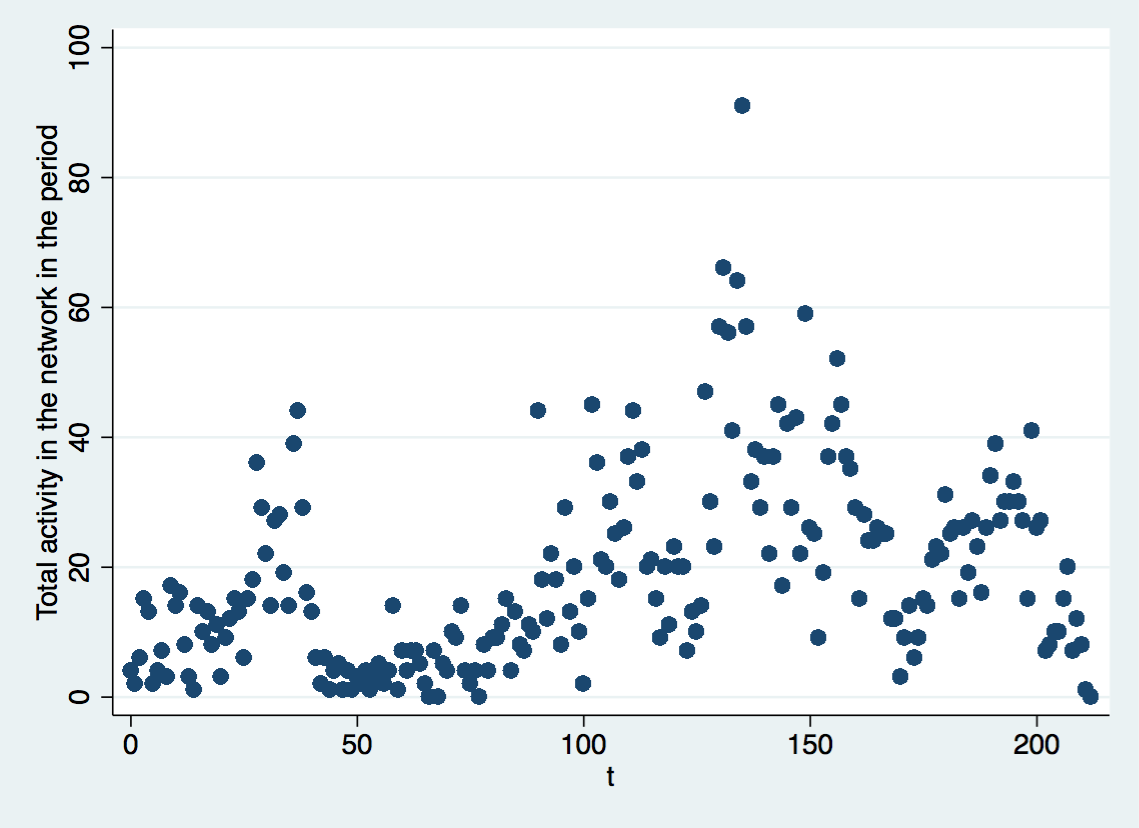
\includegraphics[width = \textwidth]{Bursty_comms_ER} 
	\caption{Weekly activity (posts + comments) in Edgeryders}
	\label{fig:burstyActivity}
\end{figure}

Figure \ref{fig:burstyActivity} refers to all activity in the network, both by ordinary users and community managers. The two are obviously correlated: a lot of what community managers do is respond to user activity. The activity of ordinary users only has a similar scatterplot.

All this points to the possibility of doing an improved version of the Kim papers, based on a computer simulation encoding a more realistic model of user behaviour. In this case, it would mainly be looking at the following hypothesis, instead of hypothesis \ref{hypothesis:intimacyWorks}:

\begin{intimacy}
	High levels of intimacy result in user disengagement, even under the new model specification.
	\label{hypothesis:newModelWorks}
\end{intimacy}

Hypothesis \ref{hypothesis:commManagersWork} would stand.

\end{document}